
\documentclass[a4paper,11pt]{article}

% Package imports
\usepackage{latexsym}
\usepackage[romanian]{babel}
\usepackage{xcolor}
\usepackage{float}
\usepackage{ragged2e}
\usepackage[empty]{fullpage}
\usepackage{wrapfig}
\usepackage{lipsum}
\usepackage{tabularx}
\usepackage{titlesec}
\usepackage{geometry}
\usepackage{marvosym}
\usepackage{verbatim}
\usepackage{enumitem}
\usepackage{fancyhdr}
\usepackage{multicol}
\usepackage{graphicx}
\usepackage{cfr-lm}
\usepackage[T1]{fontenc}
\usepackage{fontawesome5}

\usepackage[absolute]{textpos}
\setlength{\TPHorizModule}{1mm}
\setlength{\TPVertModule}{1mm}

% Color definitions
\definecolor{darkblue}{RGB}{0,0,139}

% Page layout
\setlength{\multicolsep}{0pt} 
\pagestyle{fancy}
\fancyhf{} % clear all header and footer fields
\fancyfoot{}
\renewcommand{\headrulewidth}{0pt}
\renewcommand{\footrulewidth}{0pt}
\geometry{left=1.4cm, top=0.8cm, right=1.2cm, bottom=1cm}
\setlength{\footskip}{5pt} % Addressing fancyhdr warning

% Hyperlink setup (moved after fancyhdr to address warning)
\usepackage[hidelinks]{hyperref}
\hypersetup{
    colorlinks=true,
    linkcolor=darkblue,
    filecolor=darkblue,
    urlcolor=darkblue,
}

% Custom box settings
\usepackage[most]{tcolorbox}
\tcbset{
    frame code={},
    center title,
    left=0pt,
    right=0pt,
    top=0pt,
    bottom=0pt,
    colback=gray!20,
    colframe=white,
    width=\dimexpr\textwidth\relax,
    enlarge left by=-2mm,
    boxsep=4pt,
    arc=0pt,outer arc=0pt,
}

% URL style
\urlstyle{same}

% Text alignment
\raggedright
\setlength{\tabcolsep}{0in}

% Section formatting
\titleformat{\section}{
  \vspace{-4pt}\scshape\raggedright\large
}{}{0em}{}[\color{black}\titlerule \vspace{-7pt}]

% Custom commands
\newcommand{\resumeItem}[2]{
  \item{
    \textbf{#1}{\hspace{0.5mm}#2 \vspace{-0.5mm}}
  }
}

\newcommand{\resumePOR}[3]{
\vspace{0.5mm}\item
    \begin{tabular*}{0.97\textwidth}[t]{l@{\extracolsep{\fill}}r}
        \textbf{#1}\hspace{0.3mm}#2 & \textit{\small{#3}} 
    \end{tabular*}
    \vspace{-2mm}
}

\newcommand{\resumeSubheading}[4]{
\vspace{0.5mm}\item
    \begin{tabular*}{0.98\textwidth}[t]{l@{\extracolsep{\fill}}r}
        \textbf{#1} & \textit{\footnotesize{#4}} \\
        \textit{\footnotesize{#3}} &  \footnotesize{#2}\\
    \end{tabular*}
    \vspace{-2.4mm}
}

\newcommand{\resumeProject}[4]{
\vspace{0.5mm}\item
    \begin{tabular*}{0.98\textwidth}[t]{l@{\extracolsep{\fill}}r}
        \textbf{#1} & \textit{\footnotesize{#3}} \\
        \footnotesize{\textit{#2}} & \footnotesize{#4}
    \end{tabular*}
    \vspace{-2.4mm}
}

% Organisation header with several roles listed under it
\newcommand{\resumeOrg}[2]{
\vspace{0.5mm}\item
    \begin{tabular*}{0.98\textwidth}[t]{l@{\extracolsep{\fill}}r}
        \textbf{#1} & \footnotesize{#2} \\
    \end{tabular*}
    \vspace{-1mm}
}

\newcommand{\resumeRole}[2]{
    \par\vspace{0.3mm}
    \begin{tabular*}{0.98\textwidth}[t]{l@{\extracolsep{\fill}}r}
        \textit{\footnotesize{#1}} & \textit{\footnotesize{#2}} \\
    \end{tabular*}
    \vspace{-2.4mm}
}

\newcommand{\resumeSubItem}[2]{\resumeItem{#1}{#2}\vspace{-4pt}}

\renewcommand{\labelitemi}{$\vcenter{\hbox{\tiny$\bullet$}}$}
\renewcommand{\labelitemii}{$\vcenter{\hbox{\tiny$\circ$}}$}

\newcommand{\resumeSubHeadingListStart}{\begin{itemize}[leftmargin=*,labelsep=1mm]}
\newcommand{\resumeHeadingSkillStart}{\begin{itemize}[leftmargin=*,itemsep=1.7mm, rightmargin=2ex]}
\newcommand{\resumeItemListStart}{\begin{itemize}[leftmargin=*,labelsep=1mm,itemsep=0.5mm]}

\newcommand{\resumeSubHeadingListEnd}{\end{itemize}\vspace{2mm}}
\newcommand{\resumeHeadingSkillEnd}{\end{itemize}\vspace{-2mm}}
\newcommand{\resumeItemListEnd}{\end{itemize}\vspace{-2mm}}
\newcommand{\cvsection}[1]{%
\vspace{2mm}
\begin{tcolorbox}
    \textbf{\large #1}
\end{tcolorbox}
    \vspace{-4mm}
}

\newcolumntype{L}{>{\raggedright\arraybackslash}X}%
\newcolumntype{R}{>{\raggedleft\arraybackslash}X}%
\newcolumntype{C}{>{\centering\arraybackslash}X}%


% Commands for icon sizing and positioning
\newcommand{\socialicon}[1]{\raisebox{-0.05em}{\resizebox{!}{1em}{#1}}}
\newcommand{\ieeeicon}[1]{\raisebox{-0.3em}{\resizebox{!}{1.3em}{#1}}}

% Font options
\newcommand{\headerfonti}{\fontfamily{phv}\selectfont} % Helvetica-like (similar to Arial/Calibri)
\newcommand{\headerfontii}{\fontfamily{ptm}\selectfont} % Times-like (similar to Times New Roman)
\newcommand{\headerfontiii}{\fontfamily{ppl}\selectfont} % Palatino (elegant serif)
\newcommand{\headerfontiv}{\fontfamily{pbk}\selectfont} % Bookman (readable serif)
\newcommand{\headerfontv}{\fontfamily{pag}\selectfont} % Avant Garde-like (similar to Trebuchet MS)
\newcommand{\headerfontvi}{\fontfamily{cmss}\selectfont} % Computer Modern Sans Serif
\newcommand{\headerfontvii}{\fontfamily{qhv}\selectfont} % Quasi-Helvetica (another Arial/Calibri alternative)
\newcommand{\headerfontviii}{\fontfamily{qpl}\selectfont} % Quasi-Palatino (another elegant serif option)
\newcommand{\headerfontix}{\fontfamily{qtm}\selectfont} % Quasi-Times (another Times New Roman alternative)
\newcommand{\headerfontx}{\fontfamily{bch}\selectfont} % Charter (clean serif font)

\begin{document}
\headerfontiii

% Header (kept in a fixed-size box so the page can't squeeze it under the photo)
\noindent\begin{minipage}{\textwidth}
\begin{center}
    {\Huge\textbf{Vlad-Andrei TOMICI}}
\end{center}
\vspace{-6mm}

% \begin{wrapfigure}{l}{0.25\textwidth}
%     \vspace{-20mm}
%     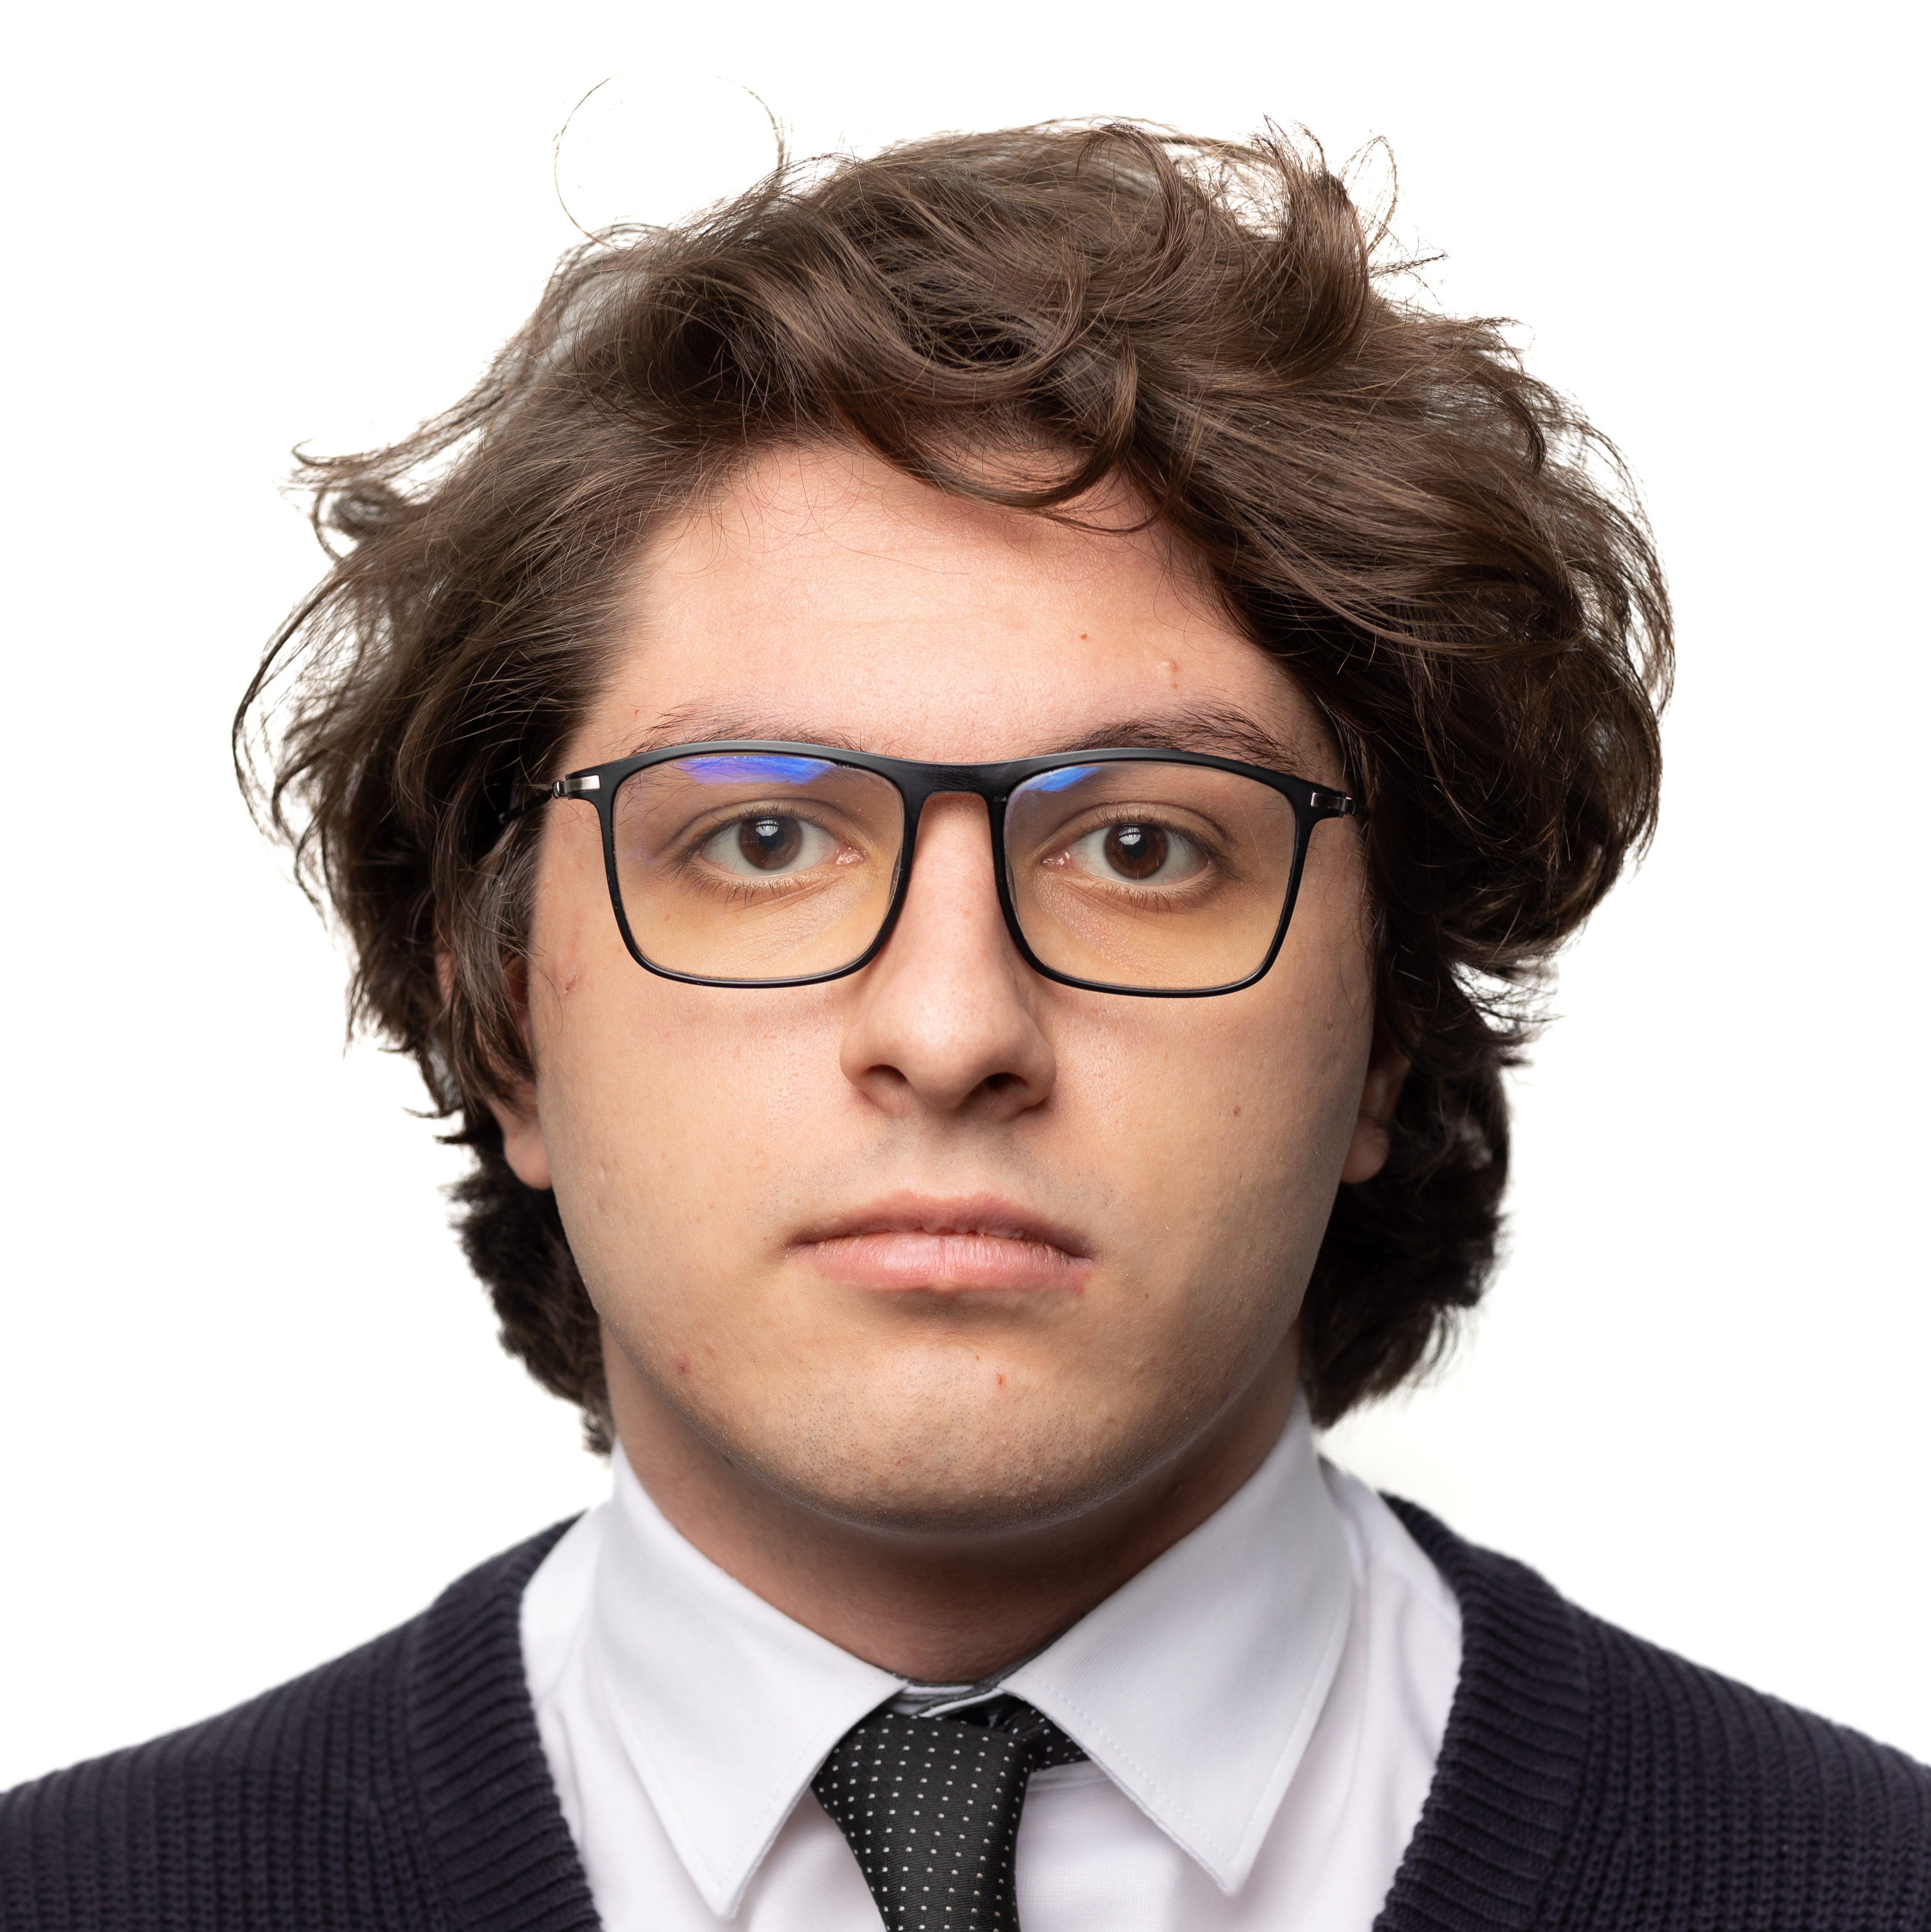
\includegraphics[width=0.25\textwidth]{STOP2008-rect.jpg}
%     \vspace{-10mm}
% \end{wrapfigure}

\begin{textblock}{30}(10, 10) % Adjust the coordinates (10, 10) as needed
    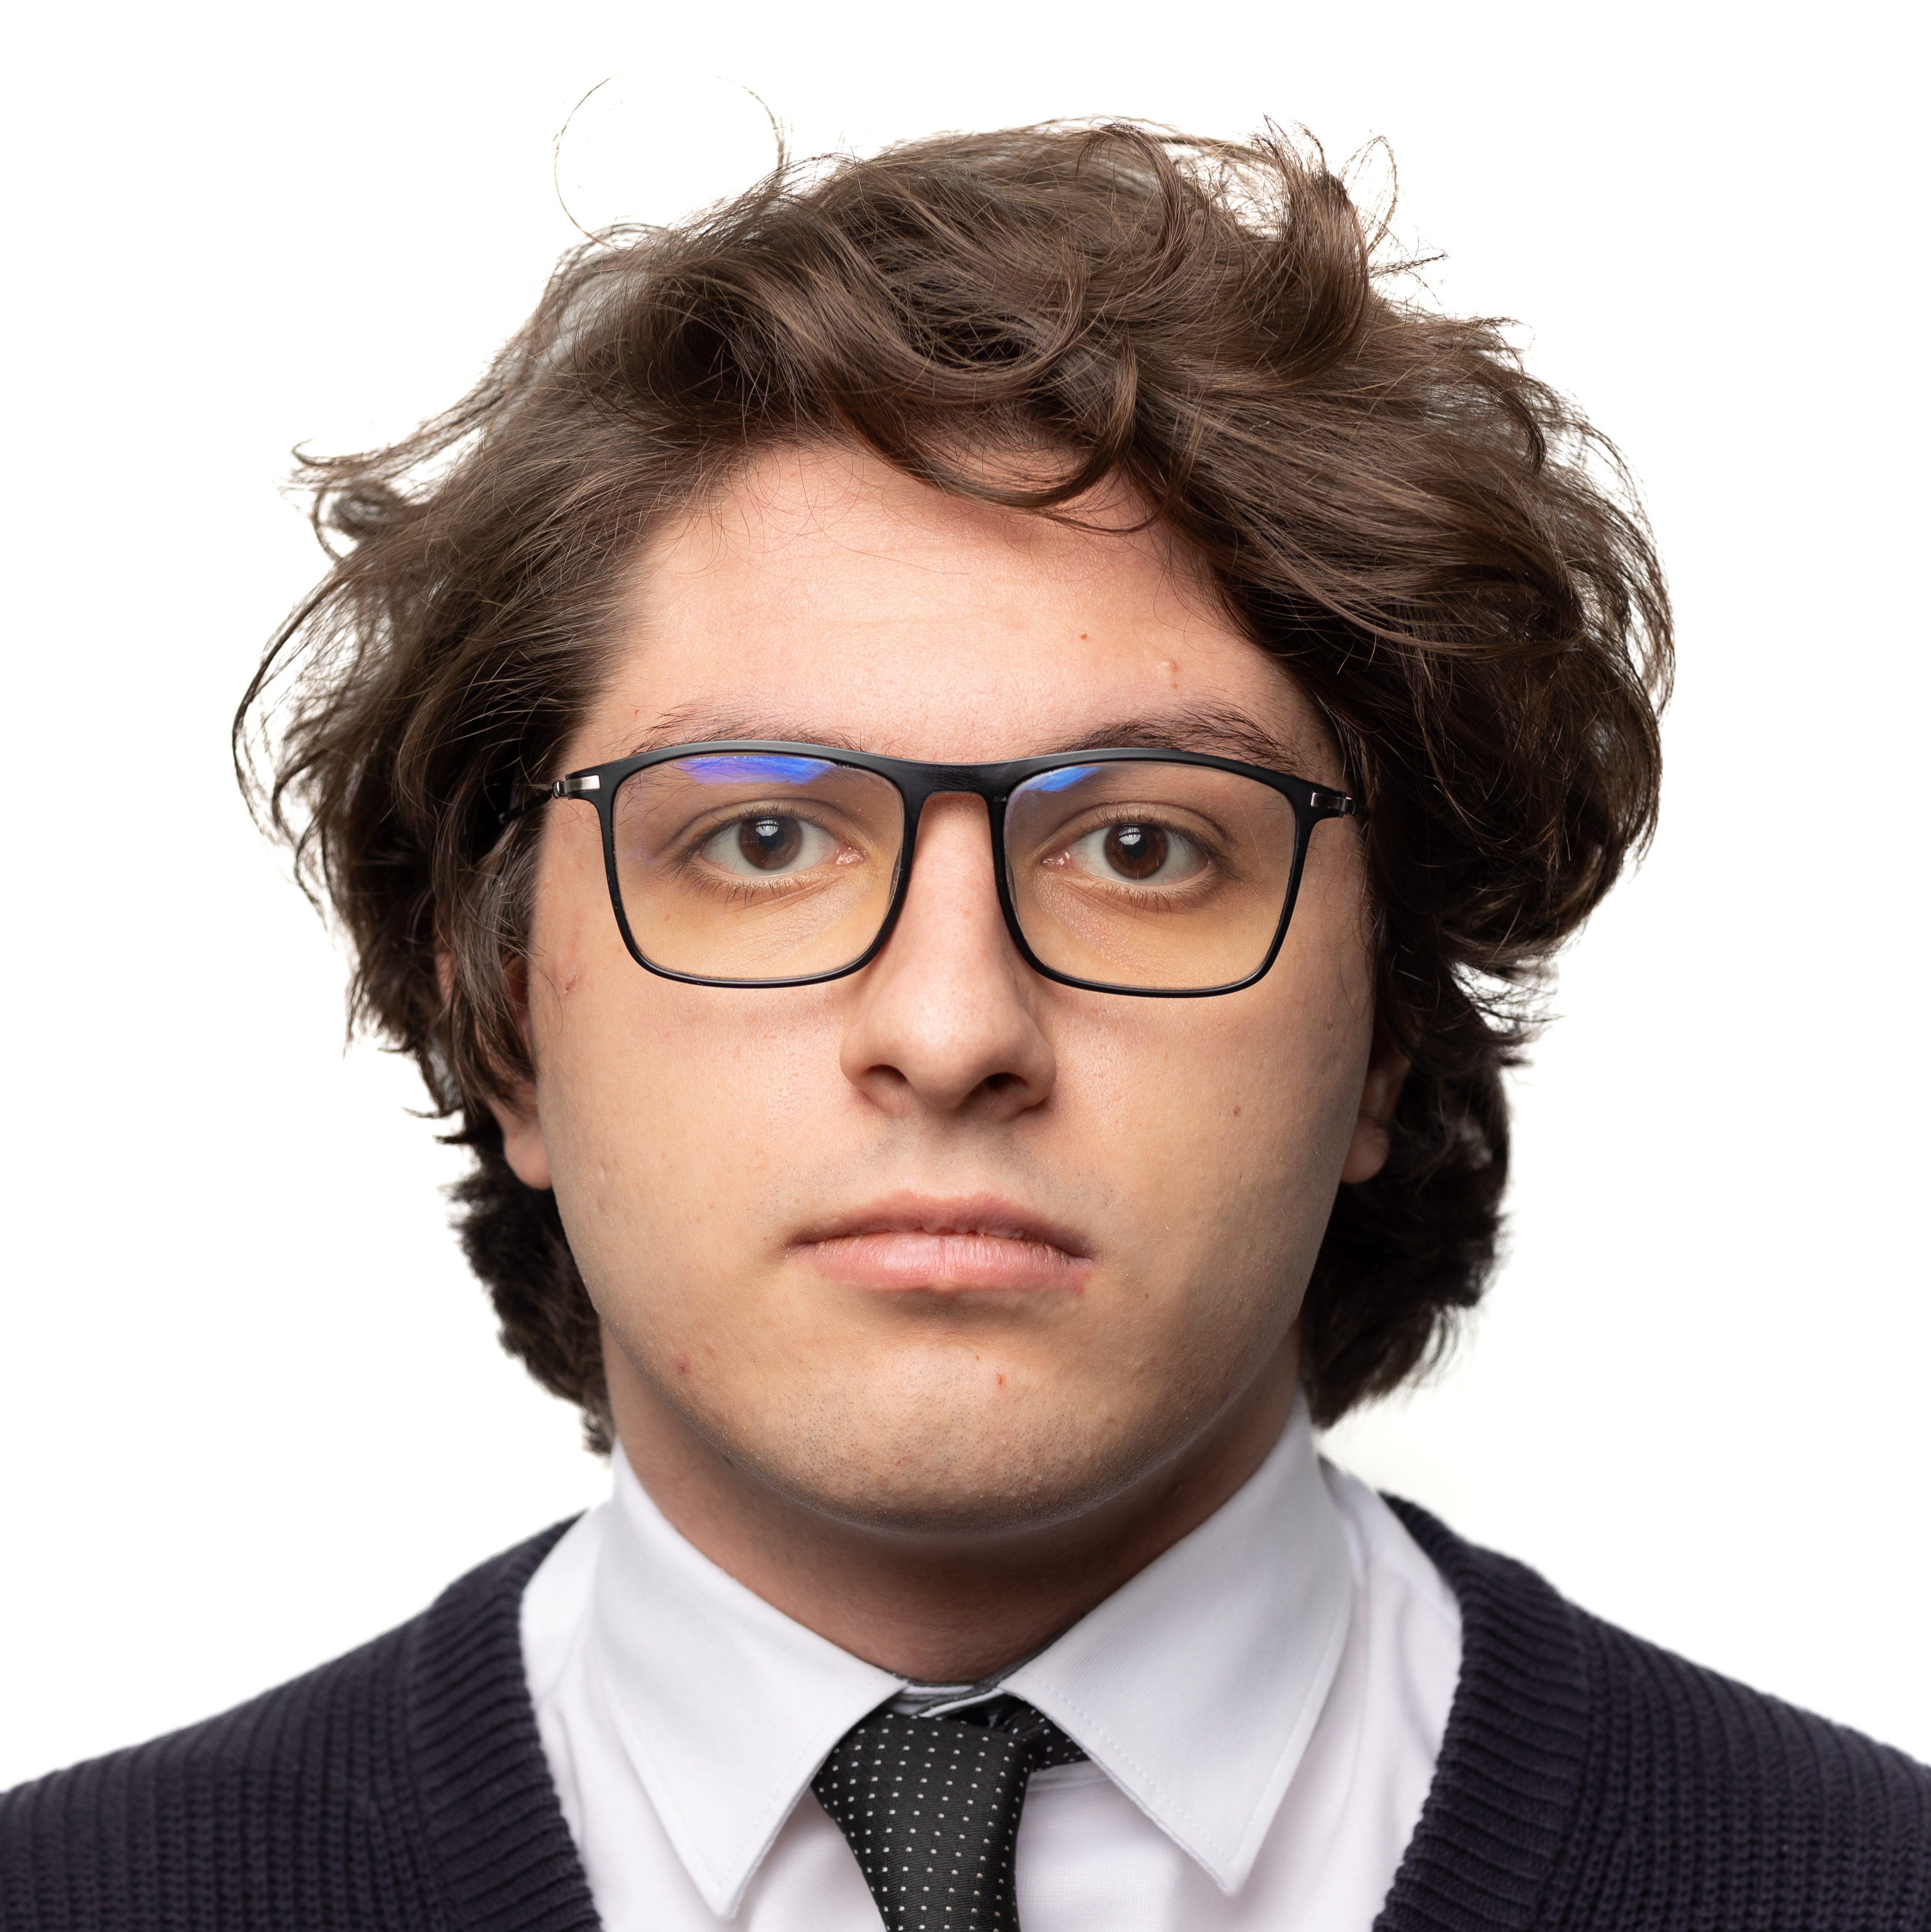
\includegraphics[width=3cm]{STOP2008-rect.jpg}
\end{textblock}

\begin{center}
    \small{
    +40-722-594-770 | \href{mailto:vladtomici@gmail.com}{vladtomici@gmail.com} | 
    \href{https://vladtomici14.github.io/}{https://vladtomici14.github.io/}
    }
\end{center}
\vspace{-6mm}

\begin{center}
    \small{
    \socialicon{\faLinkedin} \href{https://www.linkedin.com/in/vlad-tomici/}{LinkedIn Profile} | 
    \socialicon{\faGithub} \href{https://github.com/VladTomici14}{GitHub Profile}
    % \ieeeicon{\includegraphics[height=1.3em]{ieee_collabratec_icon.png}} \href{https://ieee-collabratec.ieee.org/app/p/your-profile}{your-profile} |
    % \socialicon{\faTwitter} \href{https://twitter.com/your-handle}{your-handle}
    }
\end{center}
\vspace{-6mm}
\begin{center}
    \small{Timi\c{s}oara, Romania}
\end{center}
\end{minipage}

\vspace{4mm}

\section{\textbf{About me}}
\vspace{1mm}
\small{
3rd-year Computer Engineering student with 4 years of freelance experience building \textbf{end-to-end Machine Learning solutions}: from extracting, cleaning and transforming raw datasets to training Deep Learning and Computer Vision models and integrating them into working applications. Currently an \textbf{AI Developer Intern at AUMOVIO}, building AI applications and agents on self-hosted LLMs for classification, ranking and advisory tasks that support engineering teams. Also experienced in running the infrastructure behind data-driven applications (Linux, Docker, CI/CD), and \textbf{Vice President of Internal Affairs at Liga AC}, leading industry partnerships and volunteer teams.
}
\vspace{-2mm}



\section{\textbf{Experience}}
\vspace{-0.4mm}
  \resumeSubHeadingListStart
        \resumeSubheading
        {{AUMOVIO [\href{https://www.aumovio.com/en.html}{\faIcon{globe}}]}}{Timi\c{s}oara, Romania}
          {AI Developer Intern}{Jun 2026 - Present}
        
        \resumeItemListStart
            \item Developing AI applications and agents that automate internal engineering workflows.
            \item Building classification, ranking and advisory solutions that support developers and engineers in their day-to-day work.
            \item Working with self-hosted LLMs, Jenkins pipelines and existing codebases to integrate AI tooling into development processes.
        \resumeItemListEnd
  
      \resumeOrg
        {{Liga AC [\href{https://ligaac.ro}{\faIcon{globe}}]}}{Timi\c{s}oara, Romania}
        \resumeRole{Vice President of Internal Affairs}{Sep 2026 - Present}
        
        \resumeItemListStart
            \item Industry Partnerships: Connecting our student community with the tech industry by leading discussions with private companies to secure the support that makes our projects possible.
            \item Team Coordination: Coordinating volunteer teams to ensure events run smoothly, from planning to execution.
            \item Educational Events: Supporting colleagues in creating valuable educational events for students.
        \resumeItemListEnd

        \resumeRole{Technical Department Coordinator}{Sep 2025 - Sep 2026}
        
        \resumeItemListStart
            \item Infrastructure \& DevOps: Managed a VPS Linux infrastructure, Nginx reverse proxies and MariaDB databases for high-traffic platforms.
            \item Automation \& Scalability: Built CI/CD pipelines in GitLab and containerised Docker environments for .NET, Angular and Python data processing applications.
            \item Technical Leadership: Coordinated a team of 5 Technical Project Managers, ensuring code standards and system integrations by conducting constant code reviews and 1-on-1 meetings.
        \resumeItemListEnd
      
      \resumeSubheading
          {{Freelancer}}{Remote}
          {Machine Learning and Python developer}{Mar 2022 - May 2026}
          \resumeItemListStart
            \item End-to-End ML Development: Architected and implemented complete ML solutions, covering the whole workflow from raw data processing to integrating models into functioning applications. 
            \item Computer Vision \& Deep Learning: Applied advanced techniques of image processing and Deep Learning architectures (Transfer Learning) for solving complex detection problems and classifications in dynamic environments. 
            \item Automated Data Pipelines: Developed Python optimization scripts for extracting, cleaning and transforming data sets, ensuring the input quality for model training. 
            \item Cross-Platform Integration: Collaborated on integrating AI modules in various software ecosystems (mobile and desktop), adapting algorithms according to different performance requests from the clients. 
          \resumeItemListEnd 

      \resumeSubheading
          {{Data Annotation}}{Remote}
          {Data Annotator}{Jul 2024 - Dec 2024}
          \resumeItemListStart
            \item Generating prompts and evaluating chatbot answers on programming related topics.
          \resumeItemListEnd
          
  \resumeSubHeadingListEnd
\vspace{-6mm}

\section{\textbf{Education}}
\vspace{-0.4mm}
\resumeSubHeadingListStart

\resumeSubheading
{Faculty of Automation and Computer Science}{Timi\c{s}oara, Romania}{Bachelor's degree in Computer Engineering, Department of Computers and Information Technology}{Oct 2024 - Present}

\resumeSubheading
{"Grigore Moisil" Theoretical High-School}{Timi\c{s}oara, Romania}{Secondary Education}{Sep 2020 - Jul 2024}

% \resumeSubheading
% {"Saint Mary" School Number 7}{Timi\c{s}oara, Romania}{Primary Education}{Sep 2012 - Jun 2020}

\resumeSubHeadingListEnd
\vspace{-6mm}


\section{\textbf{Skills}}
\vspace{-0.4mm}
 \resumeHeadingSkillStart
  \resumeSubItem{Programming Languages: }
    {Python (Advanced), C/C++ (Algorithms \& Embedded), C\#, Java, JavaScript, Swift, SQL}
  \resumeSubItem{Machine Learning \& Data: }
    {PyTorch, TensorFlow, Keras, Scikit-learn, Pandas, NumPy, OpenCV, Matplotlib, Jupyter Notebook, Image Processing}
  \resumeSubItem{LLMs \& AI Agents: }
    {Self-hosted LLMs (Ollama, vLLM), LangChain, Hugging Face Transformers, AI agent development, Prompt engineering}
  \resumeSubItem{DevOps \& Infrastructure: }
    {Linux, Docker, GitLab CI/CD, Jenkins, Nginx, Git}
  \resumeSubItem{Web \& Backend: }
    {Angular, .NET, MariaDB}
  \resumeSubItem{Embedded: }
    {Raspberry Pi, Arduino, Microcontrollers}
 \resumeHeadingSkillEnd


\section{\textbf{Additional Information}}
% \vspace{-0.4mm}
\small{
\textbf{Languages:} 
\resumeItemListStart
    \item Romanian \textit{(Native proficiency)}
    \item English \textit{(Professional working proficiency)} 
    \item German \textit{(Elementary proficiency)}
\resumeItemListEnd
\vspace{2mm}


\textbf{Interests:} reading, football, hiking
}


\section{\textbf{Licenses \& Certifications}}
\vspace{-0.2mm}
\resumeSubHeadingListStart

% \resumePOR{}{\href{https://certification-link-a.com}{
% \textbf{Certification A}
% }}{Month Year}

% \resumePOR{}{
% \textbf{Certifying Body:} {{\href{https://certification-link-b.com}{Certification B}}}}{Month Year}

% \resumePOR{}{
% \textbf{Certifying Body:} {{\href{https://certification-link-c.com}{Certification C}}}}{Month Year}

\resumePOR{}{\href{https://drive.google.com/file/d/1WMnR9FlJT_pPSB15GxZpJTv662y901Cq/view?usp=sharing}{
\textbf{Fundamentals of Quantum Computing and Communications Course - (RoNaQCI)}
}}{Dec 2024}

\resumePOR{}{\href{https://drive.google.com/file/d/1SCBSCP2LY4lAmFC1qx0hxTLmfbSR4jCO/view?usp=sharing}{
\textbf{Cambridge English: Advanced (CAE)}
}}{Dec 2023}

\resumePOR{}{\href{https://drive.google.com/file/d/1R3IxChVuiy-t4H5uhFsGPcKmu4DS51Wh/view?usp=sharing}{
\textbf{IC3 Certification - Global Standard 5)}
}}{Jan 2023}

\resumePOR{}{\href{https://drive.google.com/file/d/1SIY_7KhyOPoYnHBO6ikptXtp6GIHQ3-v/view?usp=sharing}{
\textbf{Cambridge English: Preliminary (PET))}
}}{May 2021}

% \resumePOR{}{\href{https://drive.google.com/file/d/1S9i8Lo0IzSALQ03V_4R9xibqxaHYoIQH/view?usp=sharing}{
% \textbf{Cambridge English: Key (KET))}
% }}{May 2018}

% \resumePOR{}{\href{https://drive.google.com/file/d/1S9SIVcP5MvXS2PAEMleNpXJqqIVLhNhJ/view?usp=sharing}{
% \textbf{Cambridge English: Flyers (YLE Flyers)}
% }}{May 2017}
 
% \resumePOR{}{\href{https://drive.google.com/file/d/1SGIGNVZuOUZEpklmOd8kzs3Kraowclcx/view?usp=sharing}{
% \textbf{Cambridge English: Movers (YLE Movers))}
% }}{May 2016}

% \resumePOR{}{\href{https://drive.google.com/file/d/1SDDmP1nszUsatExw6in075_eUzrp4SDo/view?usp=sharing}{
% \textbf{Cambridge English: Starters (YLE Starters)}
% }}{May 2015}

\resumeSubHeadingListEnd
\vspace{-6mm}

% \section{\textbf{Projects}}
% \vspace{-0.4mm}
% \resumeSubHeadingListStart

% \resumeProject
%   {Wave Propagation}
%   {Technologies used: Python, NumPy, Matplotlib, Jupyter Notebook}
%   {Dec 2024 - Jan 2025}
%   {{}[\href{https://github.com/VladTomici14/wave-propagation-visualisation}{\textcolor{darkblue}{\faGithub}}]}
% \resumeItemListStart
%   \item Developed a numerical simulation to visualize wave propagation in 2+1 dimensions.
%   \item Based on a given wave formula, the project creates an interactive 3D visualisation of the wave evolution. 
% \resumeItemListEnd

% \resumeProject
%   {DOCScan: iOS app for document scanning, text extraction and digital document management}
%   {Technologies used: Swift, SwiftUI, Python, Firebase}
%   {Mar 2024 - Jun 2024}
%   {{}[\href{https://github.com/VladTomici14/DOCScan}{\textcolor{darkblue}{\faGithub}}]}
% \resumeItemListStart
%   \item Developed using SwiftUI and Firebase for authentification and cloud storage. 
%   \item Utilizes computer vision to detect documents and enhance scanned images. 
%   \item Implemented a NLP for accurate text extraction and processing. 
%   \item Developed as a high-school graduation thesis. 
% \resumeItemListEnd

% \resumeProject
%   {Emotion recogniser}
%   {Technologies used: Python, TensorFlow, OpenCV, NumPy, Matplotlib}
%   {Apr 2022}
%   {{}[\href{https://github.com/VladTomici14/Emotion-recognition-through-transfer-learning}{\textcolor{darkblue}{\faGithub}}]}
% \resumeItemListStart
%   \item Built an emotion recognition model using the VGG16 architecture. 
%   \item Applied transfer learning and a CNN for facial expression classification. 
%   \item Developed real-time and image-based emotion detection with webcam support. 
% \resumeItemListEnd

% \resumeProject
%   {eBon: Digital receipts for a modern, eco-friendly shopping experience}
%   {Technologies used: Raspberry Pi programming, Flutter, Python, Firebase}
%   {Dec 2021}
%   {{}[\href{https://github.com/mihai-albu03/eBon}{\textcolor{darkblue}{\faGithub}}]}
% \resumeItemListStart
%   \item Built a Raspberry Pi-based hardware. 
%   \item Contributed in the development of a Flutter app for the project.
%   \item Integrated both the app and the hardware with a Firebase backend. 
%   \item Developed during the UniHack 2021 international hackathon, by me and 2 high-school colleagues. 
% \resumeItemListEnd



% \resumeProject
%   {Hand Tracking Projects: Some proof of concept scripts based on a hand tracking algorithm}
%   {Tools: [List of tools and technologies used]}
%   {Sep 2021}
%   {{}[\href{https://github.com/VladTomici14/handTrackingProjects}{\textcolor{darkblue}{\faGithub}}]}
% \resumeItemListStart
%   \item Developed [specific model/system], achieving [specific metric]
%   \item Implemented [specific feature], processing [specific volume] of data
%   \item Created [specific visualization] for [specific purpose]
%   \item Developed [specific component] for easy integration with [specific system]
% \resumeItemListEnd


% \resumeProject
%   {Rusty: a simple Raspberry Pi robot}
%   {Tools: Python, image processing, electronics, 3D modeling and printing}
%   {Oct 2018 - May 2021}
%   {{}[\href{https://github.com/VladTomici14/Rusty6}{\textcolor{darkblue}{\faGithub}}]}
% \resumeItemListStart
%   \item Designed for operations in hazardous or inaccessible areas.
%   \item Equipped with temperature \& humidity, ultrasonic and gas sensors. Powered by a solar panel and has a camera that helps in image processing with human detection.  
% \resumeItemListEnd

% \resumeSubHeadingListEnd

% \section{\textbf{Patents and Publications} \hfill \textcolor{darkblue}{\scriptsize C=Conference, J=Journal, P=Patent, S=In Submission, T=Thesis}}
% \vspace{0.2mm}
% \small{
% \begin{enumerate}[leftmargin=*, labelsep=0.5em, align=left, widest={[\textbf{S.1}]}, itemindent=0em, label={\textbf{[\arabic*]}]}]
% \item[\textbf{[C.1]}] Your Name, et al. (Year). \href{https://doi.org/XX.XXXX/XXXXXXX.XXXX.XXXXXXX}{\textbf{Title of Conference Paper}}. In \textit{Name of Conference Proceedings}, pp. XX-XX. Publisher. Date, Location. DOI: XX.XXXX/XXXXXXX.XXXX.XXXXXXX

% \item[\textbf{[S.1]}] Your Name, et al. (Year). \textbf{Title of Submitted Paper}. Manuscript submitted for publication in \textit{Journal Name}.

% \item[\textbf{[P.1]}] Inventor 1, Your Name, Inventor 3, et al. (Year). \href{https://patentoffice.gov/patent/XXXXXXXXX}{\textbf{Title of Patent}}. Patent Office, Patent No. XXXXXXXXX. Registration Date: Date, Grant Date: Date, Publication Date: Date.

% \item[\textbf{[J.1]}] Author 1, Your Name, Author 3, et al. (Year). \href{https://doi.org/XX.XXXX/XXXXX.XXXX.XXXXXXX}{\textbf{Title of Journal Article}}. \textit{Journal Name}, Vol. XX, Issue X, pp. XXX-XXX. DOI: XX.XXXX/XXXXX.XXXX.XXXXXXX
% \end{enumerate}
% }


% \section{\textbf{Honors \& Awards}}
% \vspace{-0.4mm}
% \resumeSubHeadingListStart

% \resumeProject
%   {Winner of the "Technology 4 Health (High School)" category}
%   {HackTM 2023}
%   {May 2023}
%   {{}[\href{https://github.com/VladTomici14/NeuroVault}{\textcolor{darkblue}{\faIcon{globe}}}]}

% \resumeItemListStart
%   \item Developed a web application that helps the integration of autistic people into the society by creating a more efficient way of communication between patients, specialists and patient's close people.

%   \item NeuroVault is the application that can create a profile, where the specialists can write down behaviours and consequences of the patient. In this way the future interactions between the patient and the specialists will be more efficient than ever.

%  \item Developed the back-end part of the app alongside its database using JavaScript and PHP.
% \resumeItemListEnd

% \resumeProject
%   {Intelligent Electricity Generation - 2nd place}
%   {Faculty of Electrical and Power Engineering}
%   {May 2023}
%   {{}[\href{https://drive.google.com/file/d/1lGNVWn66y1pjQws85YHQjKOu8DPgJblN/view?usp=sharing}{\textcolor{darkblue}{\faIcon{globe}}}]}
% \resumeItemListStart
%   \item Participated with WizzTech's 2022-2023 competition robot.
%   \item Award won as a member of the WizzTech Robotics Team. 
% \resumeItemListEnd

% \resumeProject
%   {AI Development, Advanced category - 3rd place}
%   {iTEC 2022}
%   {May 2022}
%   {{}[\href{https://github.com/VladTomici14/iTEC2022}{\textcolor{darkblue}{\faIcon{globe}}}]}
% \resumeItemListStart
%   \item Developed a neural network for shape and color classification.
%   \item Built a random dataset generator for geometric figures and implemented a DenseNet-based model achieving ~98\% accuracy in the training process. 
%   \item Used Python, TensorFlow, Keras and OpenCV for training and classification. 
% \resumeItemListEnd

% \resumeProject
%   {AI Development - Mention}
%   {iTEC 2021}
%   {May 2021}
%   {{}[\href{https://drive.google.com/file/d/1Rz9LomgwTDH7vVcHF6-qTt6ez0EfQ5Sy/view?usp=sharing}{\textcolor{darkblue}{\faIcon{globe}}}]}
% \resumeItemListStart
%   \item Developed the VerificAI app using the Microsoft Power Apps environment for automatising the process of management of shops' inventories.
%   % \item Skills or abilities demonstrated through this achievement
% \resumeItemListEnd

% \resumeProject
%   {Utility software and games - 1st Place}
%   {“GRIGORE MOISIL” National Software contest}
%   {May 2019}
%   {{}[\href{https://drive.google.com/file/d/1NNBqmOeLKyS263kS18LnMv4gZyOTtFkk/view?usp=sharing}{\textcolor{darkblue}{\faIcon{globe}}}]}
% \resumeItemListStart
%   \item Developed a Raspberry Pi robot that can be controlled remotely from distance and is equipped with a Pi Camera that transmits live feed from it.
% \resumeItemListEnd

% % \resumeProject
% %   {Best Hardware Project}
% %   {HackTM Oradea 2019}
% %   {Apr 2019}
% %   {{}[\href{https://competition-link.com}{\textcolor{darkblue}{\faIcon{globe}}}]}
% % \resumeItemListStart
% %   \item Specific achievement or rank in the competition
% %   \item Skills or abilities demonstrated through this achievement
% % \resumeItemListEnd

% \resumeProject
%   {Freestyle category - 3rd place}
%   {RoboTEC 2019}
%   {Apr 2019}
%   {{}[\href{https://drive.google.com/file/d/1VEAFCbDciYrWjKh9K-pOFRntG6ccpXGp/view?usp=sharing}{\textcolor{darkblue}{\faIcon{globe}}}]}
% \resumeItemListStart
%   \item Participated with a robot that was built using the Raspberry Pi platform and using some basic sensors and 4 motors. 
% \resumeItemListEnd

% \resumeSubHeadingListEnd

% \vspace{-6mm}
% \section{\textbf{Leadership Experience}}
% \vspace{-0.4mm}
% \resumeSubHeadingListStart
% \resumeProject
%   {Leadership Role A}
%   {Organization/Institution Name}
%   {Month Year - Month Year}
%   {{}[\href{https://organization-a-link.com}{\textcolor{darkblue}{\faIcon{globe}}}]}
% \resumeItemListStart
%   \item Key responsibility or achievement in this role
%   \item Quantifiable impact or improvement made during tenure
%   \item Initiative taken or project led
% \resumeItemListEnd

% \resumeProject
%   {Leadership Role B}
%   {Organization/Institution Name}
%   {Month Year - Month Year}
%   {{}[\href{https://organization-b-link.com}{\textcolor{darkblue}{\faIcon{globe}}}]}
% \resumeItemListStart
%   \item Key responsibility or achievement in this role
%   \item Quantifiable impact or improvement made during tenure
%   \item Initiative taken or project led
% \resumeItemListEnd

% \resumeSubHeadingListEnd



\section{\textbf{Volunteer Experience}}
\vspace{-0.4mm}
\resumeSubHeadingListStart

\resumeOrg
  {{WizzTech Robotics Team [\href{https://github.com/WizzTech-RO048}{\faIcon{globe}}]}}{Timi\c{s}oara, Romania}
  \resumeRole{Mentor}{Aug 2024 - Mar 2026}
\resumeItemListStart
  \item Ensuring communication with sponsors and partners. 
  \item Raised 6000\texteuro{}+ in sponsorships for team's budget.
  \item Mentoring in Java programming, robot development and 3D modelling.
  \item Ensuring a friendly and collaborative environment where each high-school student can enjoy robotics in a competitive setting.  
\resumeItemListEnd

  \resumeRole{Team Leader}{Sep 2022 - Mar 2024}
\resumeItemListStart
  \item Led a team of over 15 high school students, for 3 consecutive seasons in one of the biggest international robotics competition for high-school students: FIRST Tech Challenge. 
  \item Organised \textbf{WizzTech League Meet}: a local robotics competition with over 80 participants. Ensured everything regarding logistics, communication and refereeing. 
  \item Co-organised \textbf{Academia WizzTech}: a series of various workshops and presentations for high-schools interested in robotics.
  \item Raised 3000\texteuro{}+ in sponsorships for team's budget and ensured communication with sponsors and partners.
  \item All of this whilst being the team's main programmer. 
\resumeItemListEnd

\resumeProject
  {Trainer \& Organiser}
  {Solaris Debate Club}
  {Sep 2021 - Feb 2024}
  {{}[\href{https://acdv.ro/cluburi/}{\textcolor{darkblue}{\faIcon{globe}}}]}
\resumeItemListStart
  \item Trained and mentored over 50 high-school students for 2.5 consecutive years in World-Schools Debate format, argumentation, strategy and documentation by organising practice sessions, workshops and preparation for competitions.  
  \item Co-organised \textbf{Moisil Summer Open 2023}: a local debate competition with over 120 participants. Ensured everything regarding the logistics and funding.
\resumeItemListEnd

\resumeSubHeadingListEnd
\vspace{-6mm}

% \section{\textbf{Professional Memberships}}
% \vspace{-0.4mm}
% \resumeSubHeadingListStart
% \resumePOR{Professional Organization A}
%     {, Membership ID: XXXXXXXX}
%     {Month Year - Present}
% \resumePOR{Professional Organization B}
%     {, \href{https://membership-certificate-link.com}{Membership ID: XXXXXXXX}}
%     {Month Year - Present}
% \resumePOR{Professional Organization C}
%     {, \href{https://membership-certificate-link.com}{Membership ID: XXXXXXXX}}
%     {Month Year - Present}

% \resumeSubHeadingListEnd
% \vspace{-6mm}



% \section{\textbf{Courses}}
% \vspace{-0.4mm}
% \small{
% \resumeItemListStart
%     \item \textbf{Practical Python and OpenCV - PyImageSearch:} Blah blah blah

    
% \resumeItemListEnd

\vspace{-4mm}


% \section{\textbf{References}}
% \vspace{-0.2mm}
% \small{
% \begin{enumerate}[leftmargin=*,labelsep=2mm]
% \item \textbf{Reference Person 1}\\
%    Job Title, Department\\
%    Organization/Institution Name\\
%    Email: email1@example.com\\
%    Phone: +X-XXX-XXX-XXXX\\
%    \textit{Relationship: [e.g., Thesis Advisor, Manager, etc.]}

% \item \textbf{Reference Person 2}\\
%    Job Title, Department\\
%    Organization/Institution Name\\
%    Email: email2@example.com\\
%    Phone: +X-XXX-XXX-XXXX\\
%    \textit{Relationship: [e.g., Project Supervisor, Colleague, etc.]}

% \item \textbf{Reference Person 3}\\
%    Job Title, Department\\
%    Organization/Institution Name\\
%    Email: email3@example.com\\
%    Phone: +X-XXX-XXX-XXXX\\
%    \textit{Relationship: [e.g., Mentor, Collaborator, etc.]}
% \end{enumerate}
% }

\end{document}
